\chapter{Cronograma}
\label{c.cronograma}

O cronograma proposto para o caminhar do trabalho fica definido dentro das seguintes etapas:
\begin{itemize}
	\item[-] Etapa 1: Revisão Bibliográfica
	\item[-] Etapa 2: Análise e desenvolvimento das técnicas que serão estudadas
	\item[-] Etapa 3: Implementação computacional
	\item[-] Etapa 4: Análise de resultados e desenvolvimento da monografia
\end{itemize}

\begin{figure}[h]
\centering
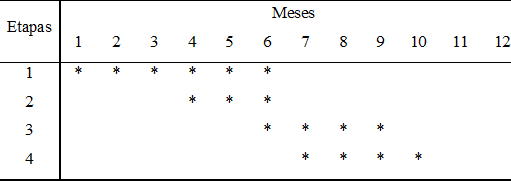
\includegraphics[scale=0.7]{figs/cronograma.png}
\label{f.cronograma}
\end{figure}





